
\documentclass[cn,hazy,blue,14pt,normal]{elegantnote}
\title{数学物理方法笔记}

\author{Jaden Feng\\冯杰骏}

\date{}

\usepackage{array}
\usepackage{physics}
\usepackage{esint}
\usepackage{amsmath}
\numberwithin{equation}{section}
\usepackage{amssymb}
\usepackage{wrapfig}
\usepackage{tikz}
\usetikzlibrary{arrows, positioning, calc, angles, quotes}

\begin{document}

\maketitle
\pagenumbering{roman}
\setcounter{page}{1}
\newpage
\begin{center}
    \Huge\textbf{{Introduction}}\\
\end{center}~\
数学物理方法笔记。
\begin{flushright}
    \begin{tabular}{c}
        Jaden Feng\\
        冯杰骏\\
        \date{\today}
    \end{tabular}
\end{flushright}

\newpage
\pagenumbering{Roman}
\setcounter{page}{1}
\tableofcontents

\newpage
\setcounter{page}{1}
\pagenumbering{arabic}

\section{复数与复变函数}
\newpage
\subsection{复数}
\begin{definition}
  虚数单位$i$
\end{definition}
$$i^2=-1 $$

\begin{definition}
  复数:
\end{definition}
$$z=x+iy$$ 
\begin{center}
	实部:$x=\text{Re}\,z$ \qquad 虚部:$y=\text{Im}\,z$ (没有 $i$ )
\end{center}

\begin{definition}
	  共轭复数:
\end{definition}
$$\overline{z} =x-iy$$
\begin{definition}
	复平面:
\end{definition}
$x$ 轴为实数轴,$y$ 轴为虚数轴,
在复平面内,用矢量 $\vec{O_z}$ 代表复数 $z=x+iy$​ ,
矢量 $\vec{O_z}$ 的长度为模(绝对值)$r=|z|=\sqrt{x^2+y^2} \geqslant 0 $。\\
\\
几个公式:
\begin{equation}\label{Complex_fundamental_inequality}
	\begin{aligned}
		|x| &\leqslant |z|, \\
		|y| &\leqslant |z|, \\
		|z| &\leqslant |x|+|y|, \\
		|z_1|+|z_2| &\geqslant |z_1 \pm z_2|, \\
		||z_1|-|z_2|| &\leqslant |z_1 \pm z_2| 
	\end{aligned}
\end{equation}

\begin{definition}
	幅角:
\end{definition}
$$\text{Arg}\ z=\theta+2k\pi , k\in\mathbb{Z}$$

幅角主值(主幅角):  $\text{arg}\ z \in (-\pi,\pi]\ or \ [0,2\pi)$\\​

若 $\text{arg}\ z \in (-\pi,\pi]$ ,有:
\begin{equation*}
    \text{arg}\ z=
\left \{
    \begin{array}{lr}
        \arctan\frac{y}{x},& x>0,\\ 
        \frac{\pi}{2},& x=0,y>0,\\
        \arctan\frac{y}{x}+\pi, & x<0,y\geqslant0,\\
        \arctan\frac{y}{x}-\pi, & x<0,y<0,\\
        -\frac{\pi}{2},& x=0,y<0.\\
    \end{array} 
\right.
\end{equation*}
\begin{note}
就是把矢量方向转到一,四象限。
\end{note}
\begin{definition}
	复数的三角形式:
\end{definition}
利用极坐标,复数还可以写成三角形式。
$$
z=x+iy=r(\cos\theta+i\,\sin\theta)
$$
$r=1$ 时,$z=\cos\theta+i\,\sin\theta$​ 称为单位复数
\begin{definition}
	复数的指数形式:
\end{definition}
由欧拉公式 $e^{i\theta}=\cos\theta+i\,\sin\theta$​​ :
$$
z=x+iy=r(\cos\theta+i\,\sin\theta)=re^{i\theta}
$$
$z=re^{i\theta}$ 称为指数形式
\begin{note}
	如何将普通形式改写为三角形式和指数形式?\\
	只需提取公因式 $r=\sqrt{x^2+y^2}$​ 即可, 需要注意的是:$r>0$ 。
\end{note}
指数形式下容易验证:
$$
\left \{
	\begin{array}{l}
		z_1\,z_2=r_1r_2e^{i(\theta_1+\theta_2)},\\
		\frac{z_1}{z_2}=\frac{r_1}{r_2}e^{i(\theta_1-\theta_2)}.
	\end{array}
\right .
$$
这表明:
$z_1\,z_2$ 对应的矢量就是把 $z_1$ 伸缩 $|z_2|$ 倍,然后幅角加 $\theta_2$ (逆时针旋转 $\theta_2$ ) ; $\frac{z_1}{z_2}$ 同理。
\begin{definition}
	棣莫弗公式:
\end{definition}
考虑复数 $z$ 的正整数次幂 $z^n$ :
\begin{equation}
	z^n=r(\cos\theta+i\,\sin\theta)^n=r^ne^{in\theta}=r^n(\cos n\theta+\sin n\theta)
\end{equation}

$r=1$ 时,得到棣莫弗公式:
\begin{equation}\label{De Moivre's formula}
(\cos\theta+i\,\sin\theta)^n=\cos n\theta+\sin n\theta
\end{equation}
\begin{example}
	计算三倍角公式
\end{example}
由棣莫弗公式\ref{De Moivre's formula}:
 $$
(\cos\theta+i\,\sin\theta)^3=\cos 3\theta+i\sin3\theta
$$
\indent 用二项式定理 $(a + b)^n = \sum\limits_{k=0}^{n} C_{n}^{k} a^{n-k} b^k$ 展开左边:

\begin{align}
	&\cos^3\theta+3i\cos^2\theta\sin\theta-3\cos\theta\sin^2\theta-i\sin^3\theta
 	\\
	=&(\cos^3\theta-3\cos\theta\sin^2\theta)+i(3\cos^2\theta\sin\theta-\sin^3\theta)
	\\
	=&\cos 3\theta+i\sin3\theta
\end{align}

实部对应实部,虚部对应虚部:

\begin{align}
 	&\cos 3\theta=\cos^3\theta-3\cos\theta\sin^2\theta=4\cos^3\theta-3\cos\theta,
	\\
	&\sin3\theta=3\cos^2\theta\sin\theta-\sin^3\theta=3\sin\theta-4\sin^3\theta.
\end{align}

\begin{note}
	两式中第二个等号都用了 $\cos^2\theta+\sin^2\theta=1$
\end{note}
\begin{definition}
	复数的n次方根:
\end{definition}
下面求复数的n次方根:
假设 $w^n=z,\;i.e.\ w=\sqrt{z}$ ,其中 $w=\rho e^{i\varphi},z=re^{i\theta}$​ ,有:
\begin{gather}
	\rho^n=r,\quad n\varphi=\theta+2k\pi;\\
\rho=\sqrt{r},\quad \varphi=\frac{\theta+2k\pi}{n}.
\end{gather}
所以:
$$
w_k=(\sqrt[n]{z})_k=\sqrt[n]{r}e^{i\frac{\theta+2k\pi}{n}}=\sqrt[n]{r}e^{i\frac{\theta}{n}}e^{i\frac{2k\pi}{n}}
$$
\begin{note}
	$z_1\,z_2$ 对应的矢量就是把 $z_1$ 伸缩 $|z_2|$ 倍,然后幅角加 $\theta_2$ (逆时针旋转 $\theta_2$ ) ; $\frac{z_1}{z_2}$ 同理。
与这句话原理相同,$e^{i\frac{2k\pi}{n}}$ 的作用效果是把 $\sqrt[n]{r}e^{i\frac{\theta}{n}}$ 的幅角加 $\frac{2k\pi}{n}$ (逆时针旋转 $\frac{2k\pi}{n}$ ) 。
$k$ 从 $0$ 开始取,取到 $n$ 时转回原点,所以共有 $n-1$ 个根。定义 $w_0=\sqrt[n]{r}e^{i\frac{\theta}{n}}$ ,可以得到 $w_k=w_0e^{i\frac{2k\pi}{n}},\quad k\in[0,n-1]$​。\\
实际计算中可以直接计算 $\frac{1}{n}$ 次方,但是要把被开方数的幅角写成 $\theta+2k\pi$ 的形式。
\end{note}


\newpage
\section{解析函数}
\newpage
\subsection{解析函数的概念以及C-R条件}

\begin{definition}
	C-R条件:
\end{definition}
直角坐标系下,对于复变函数$f(z)=u(x,y)+iv(x,y)$。
\begin{gather}
	\frac{\partial u}{\partial x}=\frac{\partial v}{\partial y},\qquad
	\frac{\partial u}{\partial y}=-\frac{\partial v}{\partial x}.
\end{gather}
称为柯西-黎曼条件(方程)。
\par 极坐标系下,对于复变函数$f(z)=u(r,\theta)+iv(r,\theta)$。
\begin{gather}
	\frac{\partial u}{\partial r}=\frac{1}{r}\frac{\partial v}{\partial \theta},\qquad
	\frac{1}{r}\frac{\partial u}{\partial \theta}=-\frac{\partial v}{\partial r}.
\end{gather}
\begin{note}
	记忆方法:$\theta$没有量纲,所以需要乘$\frac{1}{r}$让两边量纲一致。
\end{note}
\begin{theorem}
	函数$f(z)=u(x,y)+iv(x,y)$在区域$D$的内点$z=x+iy$可微的充分必要条件是$u(x,y),v(x,y)$在$(x,y)$处可微且满足C-R条件。
\end{theorem}
\begin{proof}

\end{proof}
\textbf{必要性}:i.e. $f(z)$可微$\to u,v $可微,满足C-R条件\\
如果$f(z)$在$D$内$z$点可微,那么
$$
	\Delta f(z)=f(z+\Delta z)-f(z)=f'(z)\Delta z+\rho(\Delta z)
$$
$\rho(\Delta z)$是$\Delta z$的高阶无穷小。i.e. $\lim\limits_{\Delta z\to0}\frac{\rho(\Delta z)}{\Delta z}=0$。\\ 
令$f'(z)=a+ib$,则:
\begin{align*}
	f(z+\Delta z)-f(z)&=[(u+\Delta u)+i(v+\Delta v)]-(u+iv)\\
	&=\Delta u + i \Delta v\\
	f'(z)\Delta z+\rho(\Delta z)&=a+ib(\Delta x+i\Delta y)+\rho(\Delta z)\\
	&=a\Delta x-b\Delta y+i(b\Delta x+a\Delta y)+\eta_1 + i\eta_2
\end{align*}
所以:
$$
\Delta u + i \Delta v=a\Delta x-b\Delta y+i(b\Delta x+a\Delta y)+\eta_1 + i\eta_2
$$
比较实部和虚部:
\begin{gather*}
	\Delta u=a\Delta x-b\Delta y+\eta_1,\\
	\Delta v=b\Delta x+a\Delta y+\eta_2.
\end{gather*}
由二元实函数微分的定义:
\emph{如果$f(x,y)$的自变量$x,y$在点$(x_0,y_0)$分别取得改变量$\Delta x,\Delta y$,
如果全改变量$\Delta f=f(x_0+\Delta x,y_0+\Delta y)-f(x_0,y_0)$可以表示为两个部分之和:
一部分是一个线性式,也就是$f(x,y)$的全微分$df=A\Delta x+ B\Delta y$,
另一部分是$\sqrt{{\Delta x}^2+{\Delta y}^2}$的高阶无穷小。那么就说$f(x,y)$在点$(x_0,y_0)$可微。}\\
所以$\Delta u,\Delta v$在$(x,y)$处可微。\\
分别对这两个式子求偏导数可以得到$u_x=a=v_y$,$u_y=-b=-v_x$。这就是直角坐标系下的C-R条件。\\

\par \textbf{充分性}:i.e. $u,v$可微,满足C-R条件$\to f(z)$可微\\
要证明$f(z)$可微,就要证明$\Delta f(z)$可以表示为一个线性式和一个高阶无穷小的和。
i.e. $\Delta f(z)=A(z)\Delta z+\rho(\Delta z)$\\
显然:$$\Delta f(z)=\Delta u+i\Delta v$$
又因为$u,v$可微,所以:
(这里是由二元实函数微分的定义得到的,此定义已经在必要性的证明过程中写出。)
\begin{gather*}
	\Delta u=u_x\Delta x+u_y\Delta y+\eta_1(\Delta x,\Delta y),\\
	\Delta v=v_x\Delta x+v_y\Delta y+\eta_2(\Delta x,\Delta y).
\end{gather*}
又因为$u,v$满足C-R条件,所以:
\begin{gather*}
	u_x=v_y=\alpha,\\
	u_y=-v_x=-\beta
\end{gather*}
代入$\Delta f(z)$:
\begin{align*}
	\Delta f(z)&=\Delta u+i\Delta v\\
	&=(u_x\Delta x+u_y\Delta y+\eta_1)+i(v_x\Delta x+v_y\Delta y+\eta_2)\\
	&=(\alpha+i\beta)(\Delta x+i\Delta y)+\eta_1+i\eta_2\\
	&=(\alpha+i\beta)\Delta z+\rho(\Delta z)
\end{align*}
回过头去看看复变函数微分的定义:一个线性式和一个高阶无穷小的和。i.e. $\Delta f(z)=A(z)\Delta z+\rho(\Delta z)$\\
显然只要证明$\rho$是无穷小量就可以了。(关于$z$的)\\
由公式(\ref{Complex_fundamental_inequality})的第二个式子可以得到:
$$
\left\lvert \frac{\rho}{\Delta z} \right\rvert=\left\lvert \frac{\eta_1+i\eta_2}{\Delta z} \right\rvert
\leqslant\left\lvert \frac{\eta_1}{\Delta z} \right\rvert+\left\lvert \frac{\eta_2}{\Delta z} \right\rvert
$$
当$\Delta z \to 0$时,因为$u,v$都可微,所以不等号右边两项都等于0(还是因为定义),
所以$\left\lvert \frac{\rho}{\Delta z} \right\rvert=0$,i.e. $\rho$是无穷小量。\\
综上,我们证明了$f(z)$可微。\\
同时我们还证明了:$f'(z)=\alpha+i\beta=u_x+iv_x$。\\
证毕。

\begin{example}
	举一个满足C-R条件,但是不可微的例子:
	$f(z)=\sqrt{|xy|}$在$z=0$处满足C-R条件,但是不可微。
\end{example}
函数$f(z)=\sqrt{|xy|}=u(x,y)+iv(x,y)$。于是:\\
\begin{gather*}
	u_x(0,0)=\lim_{\Delta x\to0}\frac{u(\Delta x,0)-u(0,0)}{\Delta x}=\lim_{\Delta x\to0}\frac{\sqrt{|\Delta x\cdot0|}}{\Delta x}=0=v_y(0,0),\\
	u_y(0,0)=\lim_{\Delta y\to0}\frac{u(0,\Delta y)-u(0,0)}{\Delta y}=\lim_{\Delta y\to0}\frac{\sqrt{|\Delta y\cdot0|}}{\Delta y}=0=-v_x(0,0).\\
\end{gather*}
满足C-R条件。但是:\\
\begin{equation*}
	\frac{f(\Delta z)-f(0)}{\Delta z}=\frac{\sqrt{\Delta x \cdot \Delta y}}{\Delta x+i\Delta y}
\end{equation*}
当沿$\Delta y=k\Delta x$趋近于0时,有:原式$=\frac{\sqrt{k}}{1+ik}$与$k$有关,所以原式不可微。

\begin{definition}
	解析点
\end{definition}
如果函数$\omega=f(z)$在点$z_0$的某邻域内处处可微,那么就说$z_0$是函数$\omega=f(z)$的解析点,
或者说函数$\omega=f(z)$在点$z_0$解析。

\begin{definition}
	解析函数
\end{definition}
如果区域$D$内的每一点都是函数$\omega=f(z)$的解析点,那么就说函数$\omega=f(z)$在区域$D$内解析,
或者说函数$\omega=f(z)$是区域$D$内的解析函数。

\begin{definition}
	奇点
\end{definition}
如果$f(z)$在$z_0$点不解析,但在$z_0$的邻域总有一点解析,那么就说$z_0$是$f(z)$的奇点。

\begin{example}
	$f(z)=e^x(\cos y+i\sin y)$在$z$平面上解析,而且$f'(z)=f(z)$
\end{example}

把原式展开可以知道:
$$
u(x,y)=e^x\cos y,\quad v(x,y)=e^x\sin y
$$
所以:
\begin{gather*}
	u_x=e^x\cos y,\quad u_y=-e^x\sin y\\
	v_x=e^x\sin y,\quad v_y=e^x\cos y
\end{gather*}
这几个式子证明了$u,v$的偏导数存在,又因为$u,v$都连续(初等函数的组合),所以$u,v$可微。\\
这几个式子又满足C-R条件。所以$f(z)$在$z$平面上解析。\\

\begin{example}
	由条件:
	$\left\{
	\begin{aligned}
		&u(x,y) = x^2-y^2+xy\\
		&f(i) = -1+i
		\end{aligned}
	\right.$
	求解析函数$f(z)=u+iv$
\end{example}
因为是解析函数,所以满足C-R条件:$u_x=v_y$,$u_y=-v_x$。\\
也就是:
\begin{gather*}
	2x+y=v_y,\\
	-x+2y=v_x.
\end{gather*}
从上面的第一个式子可以知道:
$$
v=\int (2x+y)dy + v(x) = 2xy+\frac{1}{2}y^2 + \varphi(x) + C
$$
\textbf{这里的$\varphi(x)$是$v$里面只有$x$的项}\\
把这个式子对$x$求导,可以得到:(这里是因为对$x$求导可以用到剩下的那个式子,所以想到的。)
$$
v_x=2y+\varphi'(x)=2y-x
$$
所以
$$
\varphi'(x)=-x\qquad\Rightarrow\qquad\varphi(x)=-\frac{1}{2}x^2
$$
所以:
$$
f(x,y)=x^2-y^2+xy+i(2xy+\frac{1}{2}y^2-\frac{1}{2}x^2+C)
$$
我们又知道,$f(i)=-1+i$,所以把$i$带进去($x=0,y=1$):
$$
-1+i=-1+i(\frac12 + C) \qquad\Rightarrow\qquad C=\frac12
$$
所以:
$$
f(x,y)=x^2-y^2+xy+i(2xy+\frac{1}{2}y^2-\frac{1}{2}x^2+\frac12)
$$
我们希望把这个式子化成$f(z)$而不是$f(x,y)$的形式。
这需要利用共轭复数。\\
我们知道
$$
z=x+iy,\quad \overline{z}=x-iy
$$
经过一些很容易的变换(两式相加,两式相减),可以得到:
$$
x=\frac{z+\overline{z}}{2},\quad y=\frac{z-\overline{z}}{2i}
$$
把这个结果带进去,可以得到:
$$
f(z)=(1+\frac i2)z^2+\frac i2
$$
\begin{note}
	这里需要注意两点:
	\begin{itemize}
		\item $\varphi(x)$是$v$里面只有$x$的项
		\item 利用共轭复数,将$f(x,y)$化成$f(z)$的形式
	\end{itemize}
\end{note}

\subsection{解析函数与调和函数的关系}
\begin{definition}
	调和函数
\end{definition}
若实函数$H(x,y)$在区域$D$内有二阶偏导数且
$$
(\frac{\partial^2}{\partial x^2} + \frac{\partial^2}{\partial y^2})H = 0,
$$
则称$H(x,y)$为$D$内的调和函数。\\
这个式子称作拉普拉斯方程。
\begin{definition}
	共轭调和函数
\end{definition}
若$D$内两个调和函数$u,v$满足C-R条件,则称它们为共轭调和函数。

\subsection{初等解析函数}
\begin{definition}
	复数域上的三角函数
\end{definition}

\begin{align}
	\cos z &= \frac{e^{iz} + e^{-iz}}{2}, \\
	\sin z &= \frac{e^{iz} - e^{-iz}}{2i},
\end{align}

\begin{definition}
	复数域上的双曲函数
\end{definition}

\begin{align}
	\sinh z &= \frac{e^z - e^{-z}}{2}, \\
	\cosh z &= \frac{e^z + e^{-z}}{2}.
\end{align}

\begin{definition}
	复数域上的根式函数
\end{definition}

$$
\omega = z^{1/n},
$$

记 $\omega = \rho e^{i\varphi}, z = re^{i\theta}$,可以推出
\begin{align*}
	\rho &= r^{1/n}, \\
\varphi &= \frac{\theta}{n} + k \frac{2\pi}{n}, k \in Z,
\end{align*}
即
$$
\omega = r^{1/n} e^{i (\frac{\theta}{n} + k \frac{2\pi}{n}) }, ~~ k = 0, 1, \cdots, n-1
$$
$k$ 的 $n$ 个取值定义了 $\omega = f(z)$ 的 $n$个单值分支。每一支的俯角都相差$\frac{2\pi}{n}$。
$$
\omega_k = (z^{1/n})_k = r^{1/n} e^{i\frac{\theta + 2k\pi}{n}}, ~~ k = 0,1,\cdots,n-1
$$

\begin{definition}
	复数域上的对数函数
\end{definition}

(以$e$为底的)对数函数是$e$指数的反函数
$$
z = e^\omega \Rightarrow \omega = Ln z,
$$
可得
$$
Ln z = \ln(re^{i(\theta + 2k\pi)}) = \ln r + i(\theta + 2k\pi), k = 0, \pm 1, \pm 2, \cdots
$$
主值支:
$$
\ln z = \ln r + i arg z,
$$
其中 $arg z$ 为 $z$ 的辐角主值,区间可定义为 $(-\pi, \pi]$ 或者 $[0,2\pi)$。

\begin{example}
	解方程$e^z = 1 + i \sqrt{3}$
\end{example}
因为$z = x + iy$,所以$e^z = e^x e^{iy}$。\\
又因为
$$
e^iy = \cos y + i \sin y,
$$
所以:
$$
e^z = e^x \cos y + i e^x \sin y = 1 + i \sqrt{3}
$$
实部对应实部,虚部对应虚部。
$$
\left \{
\begin{aligned}
	e^x \cos y &= 1, \\
	e^x \sin y &= \sqrt{3}.
\end{aligned}
\right.
$$
解这个方程组就能知道
$$
\left \{
\begin{aligned}
	x &= \ln 2, \\
	y &= \frac{\pi}{3} + 2k\pi, k \in Z.
\end{aligned}
\right.
\qquad \Rightarrow \qquad z = \ln 2 + i(\frac{\pi}{3} + 2k\pi), k \in Z.
$$

\newpage
\section{柯西定理,柯西积分}
\newpage
\subsection{复积分定义}
\begin{definition}
	复变积分
\end{definition}

$C$为起点$z_0$、终点$z_n$之间的有向曲线,$\Delta z_k = z_k - z_{k-1}$\\
定义$C$上的复变积分
$$
\int_c f(z) \dd z = \lim_{\Delta z_1, \Delta z_2, \cdots, \Delta z_n \rightarrow 0} \sum^n_{k=1} f(\zeta_k) \Delta z_k,
$$
其中 $\zeta_k$ 为 $z_{k-1}$ 到 $z_k$ 的弧段上任意一点。

\begin{definition}
	围线
\end{definition}

如果 $C$ 是逐段光滑的闭曲线,则称作是围线。
\begin{note}
	实际上按照实数的原函数,导数的规则算就行。
\end{note}
\begin{example}\label{example3.1}
试证:
$$
\oint_C \frac{ dz }{ (z-a)^n } = \left\{
\begin{aligned}
& 2\pi i, & n=1 \\
& 0, & n\neq 1, n\in Z
\end{aligned}
\right.
$$
其中 $C$ 表示以 $a$ 为中心,$\rho$ 为半径的圆周。
\end{example}

因为 $C$ 表示以 $a$ 为中心,$\rho$ 为半径的圆周,所以在 $C$ 上的复数可以表示为
$$
z = a+\rho e^{it}, ~~~ t \in [0,2\pi].
$$
取微分,则有
$$
dz = d(a+\rho e^{it}) = i\rho e^{it} dt,
$$
$n=1$ 时,有
$$
\oint_C \frac{dz}{z-a} = \int^{2\pi}_0 \frac{ i\rho e^{it} dt}{\rho e^{it}} = \int^{2\pi}_0 idt = 2\pi i,
$$
$n\neq 1$,且 $n\in Z$ 时,
$$
\oint_C \frac{dz}{(z-a)^n} = \int^{2\pi}_0 \frac{ i\rho e^{it} dt}{(\rho e^{it})^n} = i \rho^{1-n} \int^{2\pi}_0 e^{i(1-n)t}dt,
$$
再把这个式子积分号里面用欧拉公式展开:
$$
\begin{aligned}
	\oint_C \frac{dz}{(z-a)^n} &= i \rho^{1-n} \left[ \int^{2\pi}_0 \cos[(1-n)t] dt + \int^{2\pi}_0 \sin[(1-n)t] dt\right]\\
	\Rightarrow \qquad \oint_C \frac{dz}{(z-a)^n} &= 0
\end{aligned}
$$
复积分的简单性质(积分估值用到这个):
\begin{itemize}
	\item $|\int_C f(z) dz | \leq \int_C |f(z)| |dz|$
	\item $|\int_C f(z) dz | \leq Ml$,其中 $M$ 是 $|f(z)|$ 在 $C$ 上的上界,$l$ 为 $C$ 的长度。
\end{itemize}

\begin{example}
	证明:\\
	$\left | \int_{-i}^{i}  \left(x^2 + iy^2\right)\dd z \right | \leqslant \pi $,积分路径是从$-i$到$i$的右半圆周。
\end{example}	
我们知道$|\int_C f(z) dz | \leqslant \int_C |f(z)| |dz|$,所以只要证明$\int_C |f(z)| |dz| \leqslant \pi$。
也就是证明:$$|f(z)| = |x^2 + iy^2| = x^2 + y^2 \leqslant 1$$
在这个右半圆周上面,有$x^2 + y^2 = 1$,这就证明了。
\begin{note}
	这里要注意是$f(z)$的\textbf{绝对值},$x^2 + y^2$,而不是$x^2 + iy^2$。这样就很容易想明白了。
\end{note}
\subsection{柯西积分定理}
\begin{definition}\label{柯西积分定理}
	柯西积分定理
\end{definition}
如果$f(z)$在单连通域$D$内解析,$C$是$D$内任意围线,则
$$ \oint_C f(z) \dd z = 0 $$
如果$f(z)$在边界上也连续,那么这个式子还是成立。

\begin{definition}
	不定积分
\end{definition}
如果$f(z)$的单连通区域$D$内解析,则
$$
F(z) = \int^z_{z_0} f(\zeta) d\zeta
$$
只与起点$z_0$和终点$z$有关,与路径无关(通过柯西积分公式可以很容易证明)。所以选定$z_0$以后,$F(z)$ 就是关于 $z$ 的函数。其导数为
$$
F^\prime(z) = f(z),
$$
所以$F(z)$称为$f(z)$的不定积分,或原函数。
\begin{note}
	1.这里的\textbf{不定}是\textbf{不定路径}的意思\\
	2.与路径无关的证明:画两条不同的路径,这两个路径连成一个围线,在围线上的积分是零,$A + (-B) = 0 \Rightarrow A = B$。
\end{note}

\begin{definition}
	复围线上的柯西积分定理
\end{definition}

\begin{wrapfigure}[8]{r}{0.3\textwidth}
	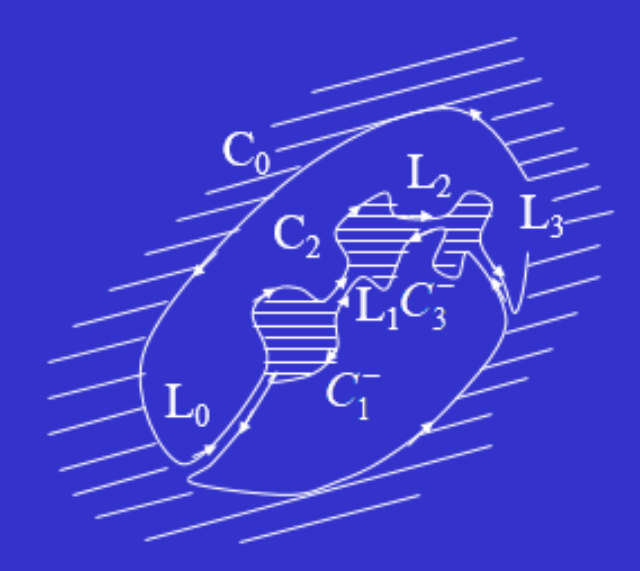
\includegraphics[width=0.3\textwidth]{./image/复围线柯西积分定理.png}
\end{wrapfigure}

如图所示,区域里面有外点,所以这是一个复连通域。把外点绕起来,然后每个圈圈连起来,就变成了如图所示的样子。
这些连起来的部分构成了 2 个单连通区域 $C_{up}, C_{down}$。根据简单围线上的柯西定理有
\begin{align*}
&\oint_{C_{up}} f(z) dz = 0, ~~~ \oint_{C_{down}} f(z) dz = 0. 
\\\Rightarrow ~~~ &\oint_{C_{up}} f(z) dz + \oint_{C_{down}} f(z) dz = 0.
\end{align*}
在极限情况下,辅助线抵消,得到
$$
C_{up} + C_{down} = C_0 + C_1 + C_2 + C_3,
$$
所以有
\begin{align*}
&\oint_{C_0} f(z) dz + \oint_{C_1} f(z) dz + \oint_{C_2} f(z)dz + \oint_{C_3} f(z) dz \\
=&\oint_{C_{up}} f(z) dz + \oint_{C_{down}} f(z) dz ~~~=~~~  0.
\end{align*}
因此,\textbf{解析函数在复围线上的积分为零。}即柯西积分定理在复围线上成立。

\begin{theorem}\label{柯西积分定理推论}
	柯西积分定理推论
\end{theorem}

\begin{wrapfigure}[5]{r}{0.25\textwidth}
	\begin{center}
		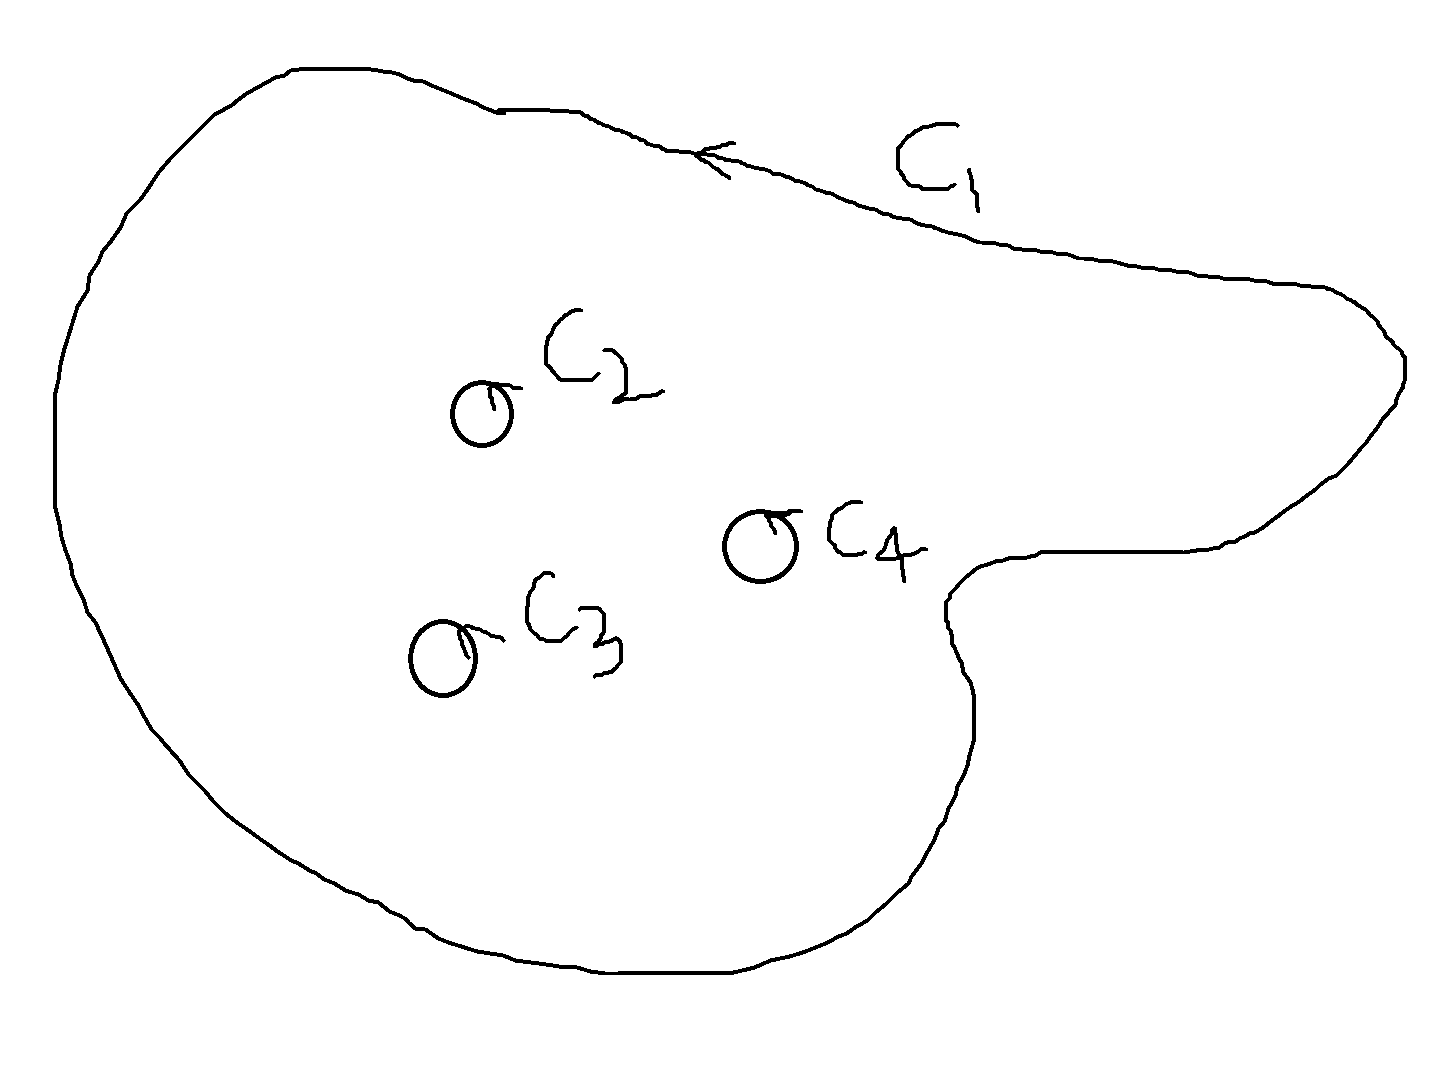
\includegraphics[width=0.25\textwidth]{./image/柯西积分定理推论.png}
	\end{center}
\end{wrapfigure}
若$f(z)$在$C_1$之内,$C_2,C_3,C_4$之外的区域解析,\\
根据复围线上的柯西积分定理,有
$$
\oint_{C_1} f(z) dz + \oint_{C^-_2} f(z) dz + \oint_{C^-_3} f(z) dz + \oint_{C^-_4} f(z) dz = 0,
$$
所以有
$$
\oint_{C_1}f(z) dz = \oint_{C_2}f(z)dz + \oint_{C_3}f(z) dz + \oint_{C_4} f(z) dz.
$$
\begin{note}
	这个的意思就是一个围线的积分等于这个围线里面所以圈圈的积分加起来。\\
	\textbf{要注意:}所有的圈圈都是同方向的,里面的圈圈要包围着奇点。
\end{note}

\begin{example}
	设$a$是围线$C$内部一点,证明
	$$
	\oint_C \frac{dz}{(z-a)^n} = \left\{
	\begin{aligned}
	2 \pi i, n=1 \\
	0, n \neq 1, n\in Z
	\end{aligned}
	\right.
	$$
\end{example}
这个题和例题(\ref{example3.1})的区别是:这个题的$C$是任意的围线,不一定是圆。\\
根据前面给出的推论(\ref{柯西积分定理推论}),
$$
\oint_C \frac{dz}{(z-a)^n} = \oint_{\gamma_\rho} \frac{dz}{(z-a)^n},
$$
其中,$\gamma_\rho$表示以$a$为圆心,以很小的$\rho$为半径($\gamma_\rho$全在$C$内部)的圆。
因为$\frac{1}{(z-a)^n}$在$C$与$\gamma_\rho$之间处处解析,所以有上面的式子。\\
接下来就和例题(\ref{example3.1})一样了。

\begin{example}\label{example3.4}
	由积分$\oint_C \frac{\dd z}{z+2}$的值证明:
	$$ \int_{0}^{\pi}\frac{1~+~2\cos\theta}{5~+~4\cos\theta}\dd \theta = 0 $$
	其中$C$是单位圆周。
\end{example}
看到这个式子是一个积分等于零,还是一个围线积分,这很容易想到用柯西积分定理。\\
$\frac{\dd z}{z+2}$在单位圆内没有奇点,所以$\oint_C \frac{\dd z}{z+2} = 0$。\\
如果能把这个式子化成下面的形式就好了
$$\int_{0}^{\pi}\frac{1~+~2\cos\theta}{5~+~4\cos\theta}\dd \theta$$
$z$是一个复数,能把复数和三角函数联系起来的就是欧拉公式$e^{i\theta} = \cos\theta + i\sin\theta$,
因为$C$是单位圆周,所以$z = e^{i\theta}$(单位圆周所以$\rho = 1$)\\
综上,所以:
\begin{align*}
&\frac{-\sin\theta~+~i\cos\theta}{\cos\theta~+~i\sin\theta~+~2}~\dd \theta\\
=~& \frac{\left(-\sin\theta~+~i\cos\theta\right)\left[(\cos\theta~+~2)~-~i\sin\theta\right]}
{\left[(\cos\theta~+~2)~+~i\sin\theta\right]\left[(\cos\theta~+~2)~-~i\sin\theta\right]}~\dd\theta\\
=~& \frac{-2\sin\theta~+~i\left(2\cos\theta~+~1\right)}{4\cos\theta~+~5}~\dd\theta
\end{align*}
因为总的积分等于零,所以虚部的积分也等于零。($\int u+iv = \int u~+~i\int v = 0+i0 = 0$)\\
也就是:
$$ \int_{0}^{2\pi}\frac{1~+~2\cos\theta}{5~+~4\cos\theta}\dd \theta = 0 $$
这样还缺少一步,因为题里的上限是$\pi$,这里是$2\pi$。那么只要证明(证明了这个就能化成$2a=0 \to a=0$)。
$$ \int_{0}^{\pi} f(\theta) \dd \theta ~=~ \int_{\pi}^{2\pi} f(\theta) \dd \theta $$
因为被积函数在这个区域里解析,所以有
$$\int_{0}^{\pi} f(\theta) \dd \theta ~=~ \int_{2\pi(0)}^{\pi} f(\theta) \dd \theta ~=~ -\int_{\pi}^{2\pi} f(\theta) \dd \theta$$
只要证明
$$\int_{\pi}^{2\pi} f(\theta) ~=~ -\int_{\pi}^{2\pi} f(\theta) \dd \theta$$
被积函数如果是偶函数,这个式子就成立了。集中注意力观察一下,果然是。\\
所以:
$$ \int_{0}^{\pi}\frac{1~+~2\cos\theta}{5~+~4\cos\theta}\dd \theta = 0 $$

\begin{example}
	计算$\oint_C \frac{dz}{z^2 -1}$,其中$C$为圆周$|z|=2$。
\end{example}
注意到
$$\frac{1}{z^2 -1} = \frac{1}{(z+1)(z-1)}$$
$\frac{1}{z+1}$和例题(\ref{example3.4})的形式差不多。
所以把原式写成这个形式:
$$
\frac{1}{z^2 -1} = \frac{1}{2}( \frac{1}{z-1} - \frac{1}{z+1} ),
$$
结合例题(\ref{example3.4})的结果(让$a = 1~,~a = -1$)有:
\begin{align*}
\oint_C \frac{\dd z}{z^2 -1} &~=~\frac{1}{2}\oint_C \frac{\dd z}{z-1} - \frac{1}{2} \oint_C \frac{\dd z}{z+1}
\nonumber\\
&~=~\frac{1}{2}(2\pi i) - \frac{1}{2}(2\pi i) ~~~=~~~ 0.
\end{align*}

\subsection{柯西积分公式}
\begin{definition}
	柯西积分公式
\end{definition}
区域$D$边界是$C$,$f(z)$在$D$内解析,在$\bar{D}=D+C$上连续,则有
\begin{equation}\label{柯西积分公式}
f(z) = \frac{1}{2\pi i} \oint_C \frac{f(\zeta)}{\zeta - z} \dd\zeta.
\end{equation}
\begin{proof}
要证明这个,只需要证明
$$\left|  \oint_C \frac{f(\zeta)}{\zeta - z} \dd\zeta - 2\pi i~f(z) \right|~\to~0$$
取$z$为圆心,半径为$\rho$(很小)的回路$\gamma_\rho$,根据复围线的柯西积分定理,
$$
\oint_C \frac{f(\zeta)}{\zeta - z} \dd \zeta
= \oint_{\gamma_\rho} \frac{f(\zeta)}{\zeta - z} \dd \zeta
$$
所以原来的式子变成
$$\left|\oint_{\gamma_\rho} \frac{f(\zeta)}{\zeta - z} d\zeta - 2\pi i~f(z)  \right|~\to~0$$
根据例题(\ref{example3.4})的结果:$2\pi i = \oint_{\gamma_\rho}\frac{1}{\zeta - z} \dd \zeta$,可以知道:
$$
\left|\oint_{\gamma_\rho} \frac{f(\zeta)}{\zeta - z} d\zeta - 2\pi i~f(z)  \right| 
= \left|\oint_{\gamma_\rho} \frac{f(\zeta)}{\zeta - z} d\zeta - f(z)\oint_{\gamma_\rho}\frac{1}{\zeta - z} \dd \zeta  \right|
$$
又因为$f(z)$和积分变量$\zeta$无关,所以可以拿到积分号里面去:
$$
\left|\oint_{\gamma_\rho} \frac{f(\zeta)}{\zeta - z} d\zeta - f(z)\oint_{\gamma_\rho}\frac{1}{\zeta - z} \dd \zeta  \right|
= \left|\oint_{\gamma_\rho} \frac{f(\zeta) - f(z)}{\zeta - z} d\zeta \right| 
$$
因为$f(\zeta)$是连续的,所以对于任意$\varepsilon>0$,只要$\rho \to 0$(充分小),就有:
$$ \left | f(\zeta)-f(z) \right | < \varepsilon $$
又因为$|\int_C f(z) dz | \leqslant \int_C |f(z)| |dz| \leqslant \int_C |M| |dz|$,$M$是$f(z)$的上界。\\
这里的$M = \frac \varepsilon \rho$($\zeta - z = \rho$(半径)\\
所以:
$$ \left|\oint_{\gamma_\rho} \frac{f(\zeta) - f(z)}{\zeta - z} d\zeta \right| < \frac \varepsilon \rho 2\pi \rho = 2 \pi \varepsilon $$
也就是:
$$ \left|\oint_{\gamma_\rho} \frac{f(\zeta)}{\zeta - z} d\zeta - 2\pi i~f(z)  \right| < 2\pi\varepsilon \to 0$$
所以
$$\oint_{\gamma_\rho} \frac{f(\zeta)}{\zeta - z} d\zeta = 2\pi i~f(z)$$
i.e.
$$ f(z) = \frac{1}{2\pi i} \oint_C \frac{f(\zeta)}{\zeta - z} \dd\zeta.$$
这个形式
$ \left|\oint_{\gamma_\rho} \frac{f(\zeta)}{\zeta - z} d\zeta - 2\pi i~f(z)  \right| < 2\pi\varepsilon \to 0$
如果觉得不太好看,在$ \left | f(\zeta)-f(z) \right | < \varepsilon $这一步把$\varepsilon$换成$\frac{\varepsilon}{2\pi}$,最终就是小于$\varepsilon$了。
\\为什么可以换?\\
因为这个$\varepsilon$是任意的,可以随便取。也就是说$\varepsilon \Leftrightarrow \frac{\varepsilon}{2\pi}$,他们都是无穷小量。\\
为什么证明了$\rho$充分时就证明了这个公式呢?\\因为我们利用柯西积分定理推论(\ref{柯西积分定理推论})得到的式子对于任意的$\rho$都成立,
所以任意的$\rho$都可以从我们最后得到的结果反向推回去。
换句话说,对于任意的$\rho$,我们的逻辑链条都是成立的(无论从前往后还是从后往前),所以我们挑一个好证的$\rho$来进行下一步。
\end{proof}

\end{document}
